
% I seguenti commenti speciali impostano:
% - applemac come codifica di input,
% - PDFLaTeX come motore di composizione;
% - Tesi.tex come documento principale;
% - il controllo ortografico italiano per l'editor.
%
% !TEX encoding = UTF-8 Unicode
% !TEX TS-program = pdflatex
% !TEX root = Tesi.tex
% !TEX spellcheck = it-IT
% ------------------------------------------------------------------------ %
%
%
% ------------------------------------------------------------------------ %
% 	PREAMBOLO
% ------------------------------------------------------------------------ %
%
\documentclass[12pt,	% 10-11-12pt (12pt preferibile)
	a4paper,		%
	twoside,		% fronte-retro
	openright,		% nuovi capitoli iniziano nella pagina dispari
	titlepage,% 	% nuova pagina dopo il titolo (necessario per frontespizio)
	]{book}
%
% ------------------------------------------------------------------------ %
%
\usepackage[T1]{fontenc}		% codifica di output
%				% N.B. richiede una distribuzione completa di LaTeX
%
\usepackage[utf8]{inputenc}		% codifica di input; anche [latin1] va bene
%				% N.B. va accordata con le preferenze dell'editor
%
\usepackage[english,italian]{babel}	% scelta lingua, sillabazione...
%				% l'ultima lingua (italiano) sarà la predefinita
%
\usepackage{microtype}		% micro-tipografia
%
% ------------------------------------------------------------------------ %
%
% 	LAYOUT - MARGINI - RILEGATURA
%
% -- AUTOMATICO
\usepackage[binding=5mm]{layaureo} 	% margini ottimizzati per l'A4; rilegatura di 5 mm
%
% -- MANUALE (Impostazioni PoliMi)
%\usepackage{geometry}
%
%\geometry{verbose,	% verbose = displays the parameter results on the terminal
%	top=43mm,	% margine superiore (PoliMi=43mm)
%	bottom=44mm,	% margine inferiore (PoliMi=44mm)
%	inner=41mm,	% margine interno pagina (PoliMi=41mm)
%	outer=32mm,	% margine esterno pagina (PoliMi=32mm)
%	bindingoffset=5mm,	% margine per la rilegatura
%	heightrounded}
%
% ------------------------------------------------------------------------ %
%
\usepackage[swapnames]{frontespizio}	% frontespizio (elegante ma non previsto al PoliMi)
%		% per includerlo nel documento bisogna:
%		% 1. compilare una prima volta Tesi.tex;
%		% 2. compilare a parte Tesi-frn.tex, generato dalla compilazione precedente;
%		% 3. compilare ancora Tesi.tex.
%		% Non è necessario fare questi passaggi altre volte
%		% se il frontespizio non è più modificato.
%
\usepackage{changepage,calc}                 % centra il frontespizio
%
\usepackage{emptypage}		% pagine vuote senza testatina e piede di pagina
%
\usepackage{indentfirst}		% rientra il primo paragrafo di ogni sezione
%
\usepackage{booktabs}		% tabelle (\toprule, \midrule, \bottomrule)
%
\usepackage{tabularx}		% tabelle di larghezza prefissata
%
\usepackage{graphicx}		% immagini
%
\usepackage[figuresright]{rotating}	% tabelle a 90 gradi
%
\usepackage{subfig}			% sottofigure, sottotabelle
%
\usepackage{caption}		% didascalie
%
\usepackage{listings}		% codici
%
\usepackage[font=small]{quoting}	% citazioni
%
\usepackage{amsmath,amssymb}	% matematica
%
\usepackage{mathtools}		% matematica
%
\usepackage{amsthm}		% matematica
%
\usepackage[output-decimal-marker={,}]{siunitx}	% SI (con separatore decimale=virgola)
%
\usepackage[italian]{varioref}		% riferimenti completi, con indicazione della pagina (\vref)
%
\usepackage{mparhack,fixltx2e}	% finezze tipografiche (bug fixes di LaTeX)
%
\usepackage{relsize}			% make text larger or smaller than the surrounding text
% 				% \larger[i] \smaller[i]
%
% ------------------------------------------------------------------------ %
%
% 	BIBLIOGRAFIA
%
% adatta lo stile delle citazioni alla lingua corrente del documento
\usepackage[autostyle,italian=guillemets]{csquotes}
%
% pacchetto biblatex
%
% STILI di citazione:
% style=numeric-comp,	<-- ufficialmente richiesto dal PoliMi (numeri tra [ ])
% style=philosophy-modern,	<-- autore-anno (meno anonimo, più immediato e più elegante)
%
\usepackage[style=philosophy-modern,	% numeric-comp oppure philosophy-modern,
	hyperref,			% riferimenti cliccabili
	backref,			% link alle pagine in cui il riferimento è citato
	natbib, 			% mantiene compatibilità con eventuali comandi natbib
	backend=biber,		% motore bibliografico (v. ArteLatex di Pantieri)
	defernumbers=true,	 	% riferimenti ordinati in ordine di comparsa
	]{biblatex}
%
\addbibresource{Bibliografia.bib}	% database bibliografico
%
% ------------------------------------------------------------------------ %
%
% Per generare effettivamente la bibliografia nel documento
% questa è la sequenza di composizione:
% 1. si compone il documento con LATEX una prima volta;
% 2. si lancia il programma Biber premendo l’apposito pulsante dell’editor;
% 3. si compone il documento altre 2 volte con LATEX (ma anche 3, NdA)
% Tale sequenza deve essere ripetuta solo se vengono fatte modifiche/aggiunte
% al database bibliografico.
%
% ------------------------------------------------------------------------ %
%
\usepackage[dvipsnames]{xcolor}	% colori - 68 colori predefiniti:
% 				% http://en.wikibooks.org/wiki/LaTeX/Colors
%
\usepackage[T1]{fontenc}
\usepackage{lmodern}

\usepackage{lipsum}			% testo fittizio
%
\usepackage{eurosym}		% simbolo dell'euro
%
\usepackage{hyperref}		% collegamenti ipertestuali
%
\usepackage{bookmark}		% gestione segnalibri del PDF
%
\usepackage{guit}			% simboli del Guit
%
\usepackage{fancyhdr}		% testatine e piede personalizzati
\setlength{\headheight}{15pt}
%
\usepackage{colortbl}		% per colorare i filetti delle tabelle
%
\usepackage[footnote,		% descrizione acronimo fatta a piè di pagina
	smaller,			% acronimo scritto con dimensione ridotta
	]{acronym}		% acronimi
%
\usepackage{multirow}		% celle tabelle alte più di una riga
%
\usepackage{pdfpages}		% inclusione di files pdf esterni
%
% ------------------------------------------------------------------------ %
% 	PREAMBOLO - SETUP
% ------------------------------------------------------------------------ %
%
% ------------------------------------------------------------------------ %
% !TEX encoding = UTF-8 Unicode
% !TEX TS-program = pdflatex
% !TEX root = Tesi.tex
% !TEX spellcheck = it-IT
% ------------------------------------------------------------------------ %
%
% ------------------------------------------------------------------------ %
% 	PREAMBOLO - SETUP
% ------------------------------------------------------------------------ %
% Comandi personali
% ------------------------------------------------------------------------ %
%
\newcommand{\myName}{Luca Maggiori}			% autore
\newcommand{\myMatricola}{783186}			% matricola
\newcommand{\myTitle}{Modello di Tesi di Laurea in \LaTeX{}}	% titolo
\newcommand{\myUni}{Politecnico di Milano}		% università
\newcommand{\myFaculty}{Scuola di Ingegneria Industriale e dell'Informazione}	% facoltà/scuola
\newcommand{\myDegree}{Ingegneria Meccanica}		% laurea
\newcommand{\myThesis}{Tesi di Laurea Magistrale}	% tipo di tesi
\newcommand{\myDepartment}{Dipartimento di Meccanica}	% dipartimento
\newcommand{\myProf}{Prof.~Charles~Dickens}		% relatore
\newcommand{\myOtherProf}{Ing.~Emilio~Salgari}		% eventuale correlatore
\newcommand{\myLocation}{Milano}			% dove
\newcommand{\myTime}{Aprile 2014}			% quando
\newcommand{\myAcademicYear}{2012--2013}		% anno accademico
\newcommand{\myLogo}{logoPoliMi}			% logo
\newcommand{\myLogoCFD}{logoPoliMiCFD}		% logo CFD :-)
\newcommand{\myUrlUni}{www.polimi.it}			% sito PoliMi
\newcommand{\myUrlFaculty}{www.ingindinf.polimi.it}	% sito Facoltà
%
% ------------------------------------------------------------------------ %
% Impostazioni di amsmath, amssymb, amsthm
% ------------------------------------------------------------------------ %
%
% un ambiente per i sistemi
\newenvironment{sistema}%
	{\left\lbrace\begin{array}{@{}l@{}}}%
	{\end{array}\right.}
%
% epsilon theta rho phi
\renewcommand{\epsilon}{\varepsilon}
\renewcommand{\theta}{\vartheta}
%\renewcommand{\rho}{\varrho}
\renewcommand{\phi}{\varphi}
%
\renewcommand{\vec}{\mathbf} 	% vettori in tondo nero
%
% ------------------------------------------------------------------------ %
% Impostazioni di biblatex
% ------------------------------------------------------------------------ %
%
% -- commentare o cancellare tutto se si desidera bibliografia standard
%
% I comandi seguenti saranno poi usati in Bibliografia.tex
% per suddividere i riferimenti bibliografici tra materiale citato
% e materiale non citato nel testo, con l'ulteriore distinzione in
% materiale cartaceo e materiale online (con link)
%
% Al termine si riportano anche pubblicazioni legate a Latex
% e alla stesura della tesi di laurea
%
\newcommand{\bibtitolocitati}{Riferimenti citati nel testo}
\newcommand{\bibtitolocitaticarta}{Pubblicazioni e Manuali}
\newcommand{\bibtitolocitatiweb}{Materiale Online}
\newcommand{\bibtitolononcitati}{Ulteriore materiale consultato}
\newcommand{\bibtitolononcitaticarta}{Pubblicazioni e Manuali}
\newcommand{\bibtitolononcitatiweb}{Materiale Online}
\newcommand{\bibtitololatex}{{\LaTeX{}}}
%
\DeclareBibliographyCategory{citati}
%
\defbibheading{citati-cartacei}{\subsection*{\bibtitolocitaticarta}}
\defbibheading{citati-web}{\subsection*{\bibtitolocitatiweb}}
\defbibheading{non-citati}{\section*{\bibtitolononcitati}}
\defbibheading{non-citati-cartacei}{\subsection*{\bibtitolononcitaticarta}}
\defbibheading{non-citati-web}{\subsection*{\bibtitolononcitatiweb}}
\defbibheading{latex}{\subsection*{\bibtitololatex}}
%
\AtEveryCitekey{\addtocategory{citati}{\thefield{entrykey}}}
%
\AtEveryBibitem{
    \clearfield{doi}
    \clearfield{eprint}
}
%
\nocite{*}	% manda in bibliografia anche tutte le opere non citate
%
% ------------------------------------------------------------------------ %
%
% Decommentare i comandi che seguono
% se si vuole ripristinare bibliografia standard
% (commentando tutto il blocco precedente)
%
%\defbibheading{bibliography}{%
%	\cleardoublepage%
%	\phantomsection%
%	\addcontentsline{toc}{chapter}{\bibname}%
%	\chapter*{\bibname\markboth{\bibname}{\bibname}}%
%	}
%
% ------------------------------------------------------------------------ %
% Impostazioni di xcolor
% ------------------------------------------------------------------------ %
%
% webcolors
\definecolor{webgreen}{rgb}{0,.5,0}
\definecolor{webbrown}{rgb}{.6,0,0}
%
% BluePolimi (colori delle presentazioni PPT del Politecnico di Milano)
\definecolor{darkbluePoliMi}{rgb}{0,0.18,0.40}	%rgb(0, 46, 103)
\definecolor{midbluePoliMi}{rgb}{0.33,0.47,0.62}	%rgb(84, 121, 157)
\definecolor{lightbluePoliMi}{rgb}{0.53,0.64,0.73}	%rgb(134, 163, 186)
\definecolor{orangePoliMi}{rgb}{1,0.59,0}		%rgb(255, 151, 0)
%
% redSapienza (rosso Sapienza)
\definecolor{redSapienza}{rgb}{0.514,0.031,0.165}	%rgb(131, 8, 42)
%
% ------------------------------------------------------------------------ %
% Impostazioni di listings
% ------------------------------------------------------------------------ %
%
\lstset{
	basicstyle=\smaller[0]\ttfamily,		% Black & White:
	keywordstyle=\color{RoyalBlue},	% keywordstyle=\color{black}\bfseries,
	commentstyle=\color{webgreen},	% commentstyle=\color{gray},
	stringstyle=\color{webbrown},		% stringstyle=\color{black},
	numbers=left,
	numberstyle=\smaller[2],
	stepnumber=1,
	numbersep=8pt,
	showspaces=false,
	showstringspaces=false,
	showtabs=false,
	breaklines=true,
	frameround=ffff,
	frame=single,
	tabsize=2,
	captionpos=t,
	breakatwhitespace=false,
	}
%
% Solution to the encoding issue
\lstset{literate=
  {á}{{\'a}}1 {é}{{\'e}}1 {í}{{\'i}}1 {ó}{{\'o}}1 {ú}{{\'u}}1
  {Á}{{\'A}}1 {É}{{\'E}}1 {Í}{{\'I}}1 {Ó}{{\'O}}1 {Ú}{{\'U}}1
  {à}{{\`a}}1 {è}{{\`e}}1 {ì}{{\`i}}1 {ò}{{\`o}}1 {ù}{{\`u}}1
  {À}{{\`A}}1 {È}{{\'E}}1 {Ì}{{\`I}}1 {Ò}{{\`O}}1 {Ù}{{\`U}}1
  {ä}{{\"a}}1 {ë}{{\"e}}1 {ï}{{\"i}}1 {ö}{{\"o}}1 {ü}{{\"u}}1
  {Ä}{{\"A}}1 {Ë}{{\"E}}1 {Ï}{{\"I}}1 {Ö}{{\"O}}1 {Ü}{{\"U}}1
  {â}{{\^a}}1 {ê}{{\^e}}1 {î}{{\^i}}1 {ô}{{\^o}}1 {û}{{\^u}}1
  {Â}{{\^A}}1 {Ê}{{\^E}}1 {Î}{{\^I}}1 {Ô}{{\^O}}1 {Û}{{\^U}}1
  {œ}{{\oe}}1 {Œ}{{\OE}}1 {æ}{{\ae}}1 {Æ}{{\AE}}1 {ß}{{\ss}}1
  {ç}{{\c c}}1 {Ç}{{\c C}}1 {ø}{{\o}}1 {å}{{\r a}}1 {Å}{{\r A}}1
  {€}{{\EUR}}1 {£}{{\pounds}}1
}
%
% Definizione ambienti per i vari linguaggi
%
\lstnewenvironment{Matlab}{\lstset{language=Matlab}}{}
%
\lstnewenvironment{C++}{\lstset{language=C++}}{}
%
\lstnewenvironment{bash}{\lstset{language=bash}}{}
%
%
% Comando per dare nome alla lista dei codici
%
\addto\captionsitalian{\renewcommand{\lstlistingname}{Codice}}
%
\addto\captionsitalian{\renewcommand{\lstlistlistingname}{Elenco dei codici}}
%
%\renewcommand{\lstlistingname}{Elenco dei codici}
%\renewcommand{\lstlistlistingname}{\lstlistingname}
%
% ------------------------------------------------------------------------ %
% Impostazioni di hyperref
% ------------------------------------------------------------------------ %
%
% per la descrizione delle varie opzioni vedere
% la guida del pacchetto hyperref
%
\hypersetup{
	%hyperfootnotes=false,
	%plainpages=false,
	%pdfpagelabels,
	colorlinks=true,
	linktocpage=true,	% true=link nei numeri pagina / false=link nel titolo
	pdfstartpage=1,
	pdfstartview=FitV,
	breaklinks=true,
	pageanchor=true,
	pdfpagemode=UseOutlines,
	%bookmarksnumbered,
	%bookmarksopen=true,
	bookmarksopenlevel=1,
	hypertexnames=true,
	pdfhighlight=/O,
	urlcolor=webbrown,		% colore dei link a pagine web
	linkcolor=RoyalBlue,		% colore dei collegamenti nel testo
	citecolor=webgreen,		% colore delle citazioni
	pdftitle={\myTitle},		% da qui in poi compilazione metadati
	pdfauthor={\textcopyright\ \myName, \myUni},
	pdfsubject={},
	pdfcreator={pdfLaTeX},
	pdfproducer={LaTeX with hyperref},
	pdfkeywords={polimi,
		tesi,
		latex,
		laurea,
		dottorato,
		scribd},
}
%
% comando per inviare mail
\newcommand{\mail}[1]{\href{mailto:#1}{\texttt{#1}}}
%
% Si possono avere tutti i collegamenti in nero e senza riquadri
% scrivendo semplicemente:
% \hypersetup{hidelinks}
%
% ------------------------------------------------------------------------ %
% Impostazioni di graphicx
% ------------------------------------------------------------------------ %
%
% Elenco dei percorsi in cui saranno cercate le immagini da inserire
%
% In questo modo non è necessario specificare il percorso relativo
% dell'immagine all'interno di \includegraphics{}, ma solo il nome.
%
% N.B. assicurarsi che non siano presenti più immagini
% con lo stesso nome.
%
\graphicspath{
	{Immagini/}
	{Immagini/Introduzione/}
	{Immagini/ProveSperimentali/}
	{Immagini/ProveSperimentali/Subfolder1/}
	{Immagini/ProveSperimentali/Subfolder2/}
	{Immagini/AnalisiNumeriche/}
	}
%
% ------------------------------------------------------------------------ %
% Impostazioni di caption
% ------------------------------------------------------------------------ %
%
\captionsetup{tableposition=top,
	figureposition=bottom,
	font=small,
	format=hang,
	labelfont=bf}
%
% ------------------------------------------------------------------------ %
% Impostazioni di fancyhdr
% ------------------------------------------------------------------------ %
%
% Impostazioni preferibili, ma NON del tutto adeguate alle norme POLIMI
% N.B. si possono usare queste impostazioni senza problemi anche per il PoliMi.
%
\pagestyle{fancy}			% sostituisce \pagestyle{header} standard
%
%\renewcommand{\chaptermark}[1]{	% ridefinisce indicazione capitolo
%	\markboth{\chaptername\ \thechapter.\ #1}{}}
%
\makeatletter 			% necessary for using \@chapapp
\renewcommand{\chaptermark}[1]{	% ridefinisce indicazione capitolo
  \markboth{\@chapapp\ \thechapter.\ #1}{}} % distinzione 'Capitolo' / 'Appendice'
\makeatother
%
\renewcommand{\sectionmark}[1]{	% ridefinisce indicazione sezione
	\markright{\thesection.\ #1}}
%
\fancyhf{}				% svuota testatine e piede
%
\fancyhead[LE,RO]{\bfseries\thepage}	% numero pagine in alto
%
\fancyhead[LO]{\bfseries\rightmark}	% info sezione nelle pag. dispari
%
\fancyhead[RE]{\bfseries\leftmark}	% info capitolo nelle pag.pari
%
\renewcommand{\headrulewidth}{0.4pt}	% spessore linea header
%
\renewcommand{\footrulewidth}{0pt}	% spessore linea footer (0pt=nascosta)
%
\fancypagestyle{plain}{				% ridefinizione stile inizio capitolo
		\fancyhead{}			% header vuoto
		\fancyfoot[C]{\bfseries\thepage}		% numeri in grassetto al centro
		\renewcommand{\headrulewidth}{0pt}	% no linea
		}
%
% ------------------------------------------------------------------------ %
%
% Impostazioni maggiormente in linea con le norme POLIMI
% (decommentare l'intero blocco e commentare il blocco precedente)
%
% N.B. si possono usare le impostazioni precedenti senza problemi anche
% per il PoliMi (e infatti io ho usato le precedenti). Il mio consiglio è di
% usare, tra le 2 versioni proposte, quella sopra.
%
%\pagestyle{fancy}			% sostituisce \pagestyle{header} standard
%%
%\makeatletter 			% necessary for using \@chapapp
%\renewcommand{\chaptermark}[1]{%
%  \markboth{\@chapapp\ \thechapter.\ #1}{}} % distinzione 'Capitolo' / 'Appendice'
%\makeatother
%%
%\fancyhf{}				% svuota testatine e piede
%%
%\fancyfoot[LE,RO]{\bfseries\thepage}	% numero pagine in basso
%%
%\fancyhead[RO]{\bfseries\leftmark}	% info capitolo pagine dispari
%%
%\fancyhead[LE]{\bfseries\leftmark}	% info capitolo pagine pari
%%
%\renewcommand{\headrulewidth}{0.4pt}	% spessore linea header
%%
%\renewcommand{\footrulewidth}{0pt}	% spessore linea footer (0pt=nascosta)
%%
%\fancypagestyle{plain}{				% ridefinizione stile inizio capitolo
%		\fancyhf{}				% header e footer azzerati
%		\fancyfoot[C]{\bfseries\thepage}		% numero di pagina al centro
%		\renewcommand{\headrulewidth}{0pt}	% no linea header
%		}
%
% ------------------------------------------------------------------------ %
% Impostazioni degli acronimi
% ------------------------------------------------------------------------ %
%
% descrizione acronimi GIUSTIFICATA
\makeatletter
\def\bflabel#1{{\textbf{\textsf{#1}}\hfill}}
\renewenvironment{AC@deflist}[1]%
{\ifAC@nolist%
\else%
\begin{list}{}%
{\settowidth{\labelwidth}{\textbf{\textsf{#1}}}%
\setlength{\leftmargin}{\labelwidth}%
\addtolength{\leftmargin}{\labelsep}%
\renewcommand{\makelabel}{\bflabel}}%
\fi}%
{\ifAC@nolist%
\else%
\end{list}%
\fi}%
\makeatother
%
% ------------------------------------------------------------------------ %
% Altro
% ------------------------------------------------------------------------ %
%
% Gradiente
\newcommand{\gradiente}[1]{$\nabla #1$}
%
% puntini di omissione [...]
\newcommand{\omissis}{[\dots\negthinspace]}
%
% Eccezioni all'algoritmo di sillabazione
\hyphenation{OpenFOAM}
\hyphenation{Matlab}
\hyphenation{bash}
%
% ------------------------------------------------------------------------ %
% Finezze tipografiche per il Politecnico di Milano
% ------------------------------------------------------------------------ %
%
% Le seguenti modifiche possono essere commentate
% o adeguate ad un'altra università (es. 'Yale Blue'
% per l'università di Yale, 'Rosso Sapienza' per La Sapienza..)
%
% Filetti tabelle colorati
\arrayrulecolor{darkbluePoliMi}
%
%
% Righe delle note a piè di pagina colorate
\renewcommand{\footnoterule}{%
  \kern -3pt
  {\color{darkbluePoliMi} \hrule width 0.4\textwidth}
  \kern 2.6pt
}
%
% ------------------------------------------------------------------------ %		% file con le impostazioni personali
%
%
% ------------------------------------------------------------------------ %
% 	BEGIN DOCUMENT
% ------------------------------------------------------------------------ %
%
\begin{document}
%
% ------------------------------------------------------------------------ %
% 	FRONTMATTER
% ------------------------------------------------------------------------ %
%
\frontmatter
%
%
% --------- CANCELLARE o COMMENTARE ---------------- %
% ------------------------------------------------------------------------ %
% !TEX encoding = UTF-8 Unicode
% !TEX TS-program = pdflatex
% !TEX root = ../Tesi.tex
% !TEX spellcheck = it-IT
% ------------------------------------------------------------------------ %
%
% ------------------------------------------------------------------------ %
% 	FRONTESPIZIO
% ------------------------------------------------------------------------ %
%
%
\pdfbookmark[1]{Frontespizio}{Frontespizio}
%
% ------------------------------------------------------------------------ %
% Frontespizio con pacchetto 'frontespizio'
% ------------------------------------------------------------------------ %
%
\begin{frontespizio}
%
%
% rinomino Matricola in Matr
\Preambolo{\renewcommand{\frontsmallfont}[1]{\small Matr.}}
%
% modifico i margini {sinistro}{basso}{destro}{alto}
\Margini{1.5cm}{1.5cm}{1.5cm}{1.5cm}
%
\Istituzione{Politecnico di Milano}
%
\Logo[2.5cm]{Immagini/logoPoliMi}
%
\Divisione{Scuola di Ingegneria Industriale e dell'Informazione}
%
%\Dipartimento{Meccanica}
%
\Corso{mathematical Engineering - Ingegneria Matematica}
%
\Titoletto{Tesi di Laurea Magistrale}
%
\Titolo{Modello di Tesi di Laurea in \LaTeX{}}
%
\Candidato[944476]{Fabrizio Bernardi}
%
\Relatore{Prof.~Riccardo~Sacco}
%
\Correlatore{Dott.~Francesco~Papaleo}
%
\Annoaccademico{2021-2022}
%
\Punteggiatura{}
%
\Rientro{1cm}
%
%
\end{frontespizio}
%
% ------------------------------------------------------------------------ %		% frontespizio figo ma non ufficiale al PoliMi
% non c'entra nulla con la tesi vera e propria
\cleardoublepage
% ------------------------------------------------------------------------ %
%
% Frontespizio ufficiale del Politecnico di Milano
%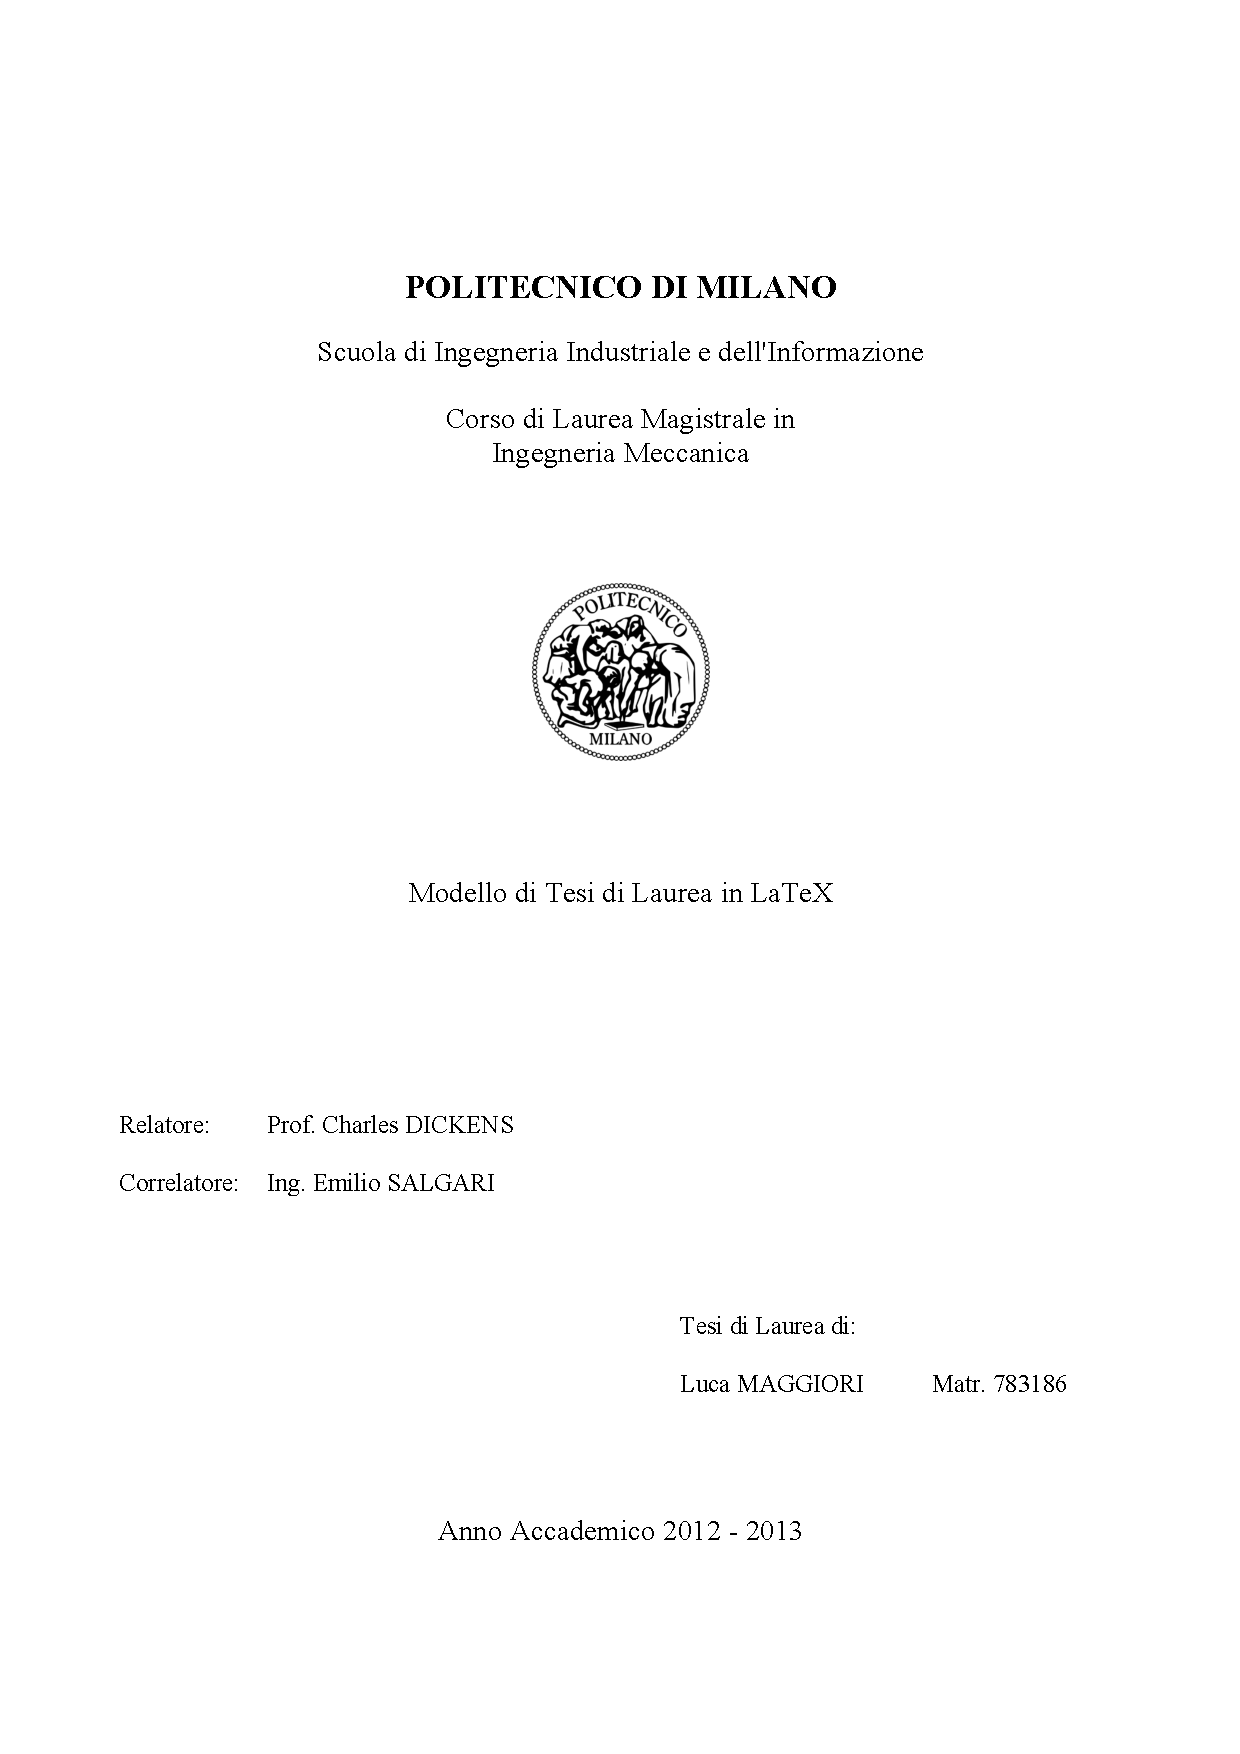
\includepdf{Frontespizio-Official-Word.pdf}
%
%% ------------------------------------------------------------------------ %
% !TEX encoding = UTF-8 Unicode
% !TEX TS-program = pdflatex
% !TEX root = ../Tesi.tex
% !TEX spellcheck = it-IT
% ------------------------------------------------------------------------ %
%
% ------------------------------------------------------------------------ %
% 	COLOPHON
% ------------------------------------------------------------------------ %
%
\clearpage
%
\phantomsection
%
\thispagestyle{empty}
%
\pdfbookmark[1]{Colophon}{Colophon}
%
% ------------------------------------------------------------------------ %
%
\hfill
%
\vfill
%
% ------------------------------------------------------------------------ %
%
\noindent\myName:
%
\textit{\myTitle} \textbar\
%
\myThesis\ in \myDegree, \myUni.
%
\\
%
\textcopyright\ Copyright \myTime.

\vspace{0.5cm}
\hrule
\bigskip

\noindent{\myUni}: \\
\href{http://\myUrlUni}{\myUrlUni}

\medskip
\noindent{\myFaculty}: \\
\href{http://\myUrlFaculty}{\myUrlFaculty}
%
% ------------------------------------------------------------------------ %
%
% ------------------------------------------------------------------------ %
% !TEX encoding = UTF-8 Unicode
% !TEX TS-program = pdflatex
% !TEX root = ../Tesi.tex
% !TEX spellcheck = it-IT
% ------------------------------------------------------------------------ %
%
% ------------------------------------------------------------------------ %
% 	RINGRAZIAMENTI
% ------------------------------------------------------------------------ %
%
\cleardoublepage
%
\phantomsection
%
\pdfbookmark{Ringraziamenti}{ringraziamenti}
%
\chapter*{Ringraziamenti}
%
\lipsum[1]

\medskip

Desidero inoltre ringraziare esplicitamente:
\begin{description}
\item[{\scshape Esplicito1}] per vari motivi;
\item[{\scshape Esplicito2}] per altri motivi;
\item[{\scshape Esplicito3}] per puro piacere, senza particolari motivi.
\end{description}
%

\bigskip
 
\noindent\textit{\myLocation, \myTime}
\hfill L.~M.
%
% ------------------------------------------------------------------------ %
%
% ------------------------------------------------------------------------ %
% !TEX encoding = UTF-8 Unicode
% !TEX TS-program = pdflatex
% !TEX root = ../Tesi.tex
% !TEX spellcheck = it-IT
% ------------------------------------------------------------------------ %
%
% ------------------------------------------------------------------------ %
% 	DEDICA
% ------------------------------------------------------------------------ %
%

%
\phantomsection
%
\thispagestyle{empty}
%
\pdfbookmark{Dedica}{Dedica}
%
\vspace*{\stretch{1}}
%
\begin{flushright}
\textit{a te,\\ovunque tu sia,\\e qualunque percorso di vita tu abbia intrapreso.}
\end{flushright}
%
\vspace{\stretch{2}}
%
% ------------------------------------------------------------------------ %
%
% ------------------------------------------------------------------------ %
% !TEX encoding = UTF-8 Unicode
% !TEX TS-program = pdflatex
% !TEX root = ../Tesi.tex
% !TEX spellcheck = it-IT
% ------------------------------------------------------------------------ %
%
% ------------------------------------------------------------------------ %
% 	INDICI
% ------------------------------------------------------------------------ %
%

%
% ------------------------------------------------------------------------ %
%
% Indice Generale
%
\pdfbookmark{\contentsname}{tableofcontents}
%
\setcounter{tocdepth}{2}
%
\tableofcontents
%

% ------------------------------------------------------------------------ %
%
% Indice delle Figure
%
\phantomsection
%
\pdfbookmark{\listfigurename}{lof}
%
\listoffigures
%

%
% ------------------------------------------------------------------------ %
%
% Indice delle Tabelle
%
\phantomsection
%
\pdfbookmark{\listtablename}{lot}
%
\listoftables
%

%
% ------------------------------------------------------------------------ %
%
% Indice dei Listati di Programma
%
\phantomsection
%
\pdfbookmark{\lstlistlistingname}{lol}
%
\lstlistoflistings
%

%
% ------------------------------------------------------------------------ %
%
% ------------------------------------------------------------------------ %
% !TEX encoding = UTF-8 Unicode
% !TEX TS-program = pdflatex
% !TEX root = ../Tesi.tex
% !TEX spellcheck = it-IT
% ------------------------------------------------------------------------ %
%
% ------------------------------------------------------------------------ %
% 	SOMMARIO + ABSTRACT
% ------------------------------------------------------------------------ %
%
\cleardoublepage
%
\phantomsection
%
\pdfbookmark{Sommario}{Sommario}
%
% ------------------------------------------------------------------------ %
% consento presenza di più capitoli nella stessa pagina
\begingroup
%\let\clearpage\relax
\let\cleardoublepage\relax
\let\cleardoublepage\relax
% ------------------------------------------------------------------------ %
%
\chapter*{Sommario}
%
\lipsum[1-2]

\medskip
%
\noindent \textbf{Parole chiave:} 
PoliMi,
Tesi,
LaTeX,
Scribd
%
\clearpage
%\vfill
%
% ------------------------------------------------------------------------ %
%
\selectlanguage{english}
%
\pdfbookmark{Abstract}{Abstract}
%
\chapter*{Abstract}
%
Text of the abstract in english\dots\\
\lipsum[1-2]

\medskip
%
\noindent \textbf{Keywords:} 
PoliMi,
Master Thesis,
LaTeX,
Scribd
%
% ------------------------------------------------------------------------ %
%
\selectlanguage{italian}
%
\endgroup			
%
%\vfill
%
% ------------------------------------------------------------------------ %
%
\cleardoublepage
%
% ------------------------------------------------------------------------ %
% 	MAINMATTER
% ------------------------------------------------------------------------ %
%
\mainmatter
%
% ------------------------------------------------------------------------ %
% !TEX encoding = UTF-8 Unicode
% !TEX TS-program = pdflatex
% !TEX root = ../Tesi.tex
% !TEX spellcheck = it-IT
% ------------------------------------------------------------------------ %
%
% ------------------------------------------------------------------------ %
% 	INTRODUZIONE
% ------------------------------------------------------------------------ %
%
\cleardoublepage
%
\phantomsection
%
\addcontentsline{toc}{chapter}{Introduzione}
%
\chapter*{Introduzione}
%
\markboth{Introduzione}{Introduzione}	% headings
%
\label{cap:introduzione}
%
% ------------------------------------------------------------------------ %
%
Due esempi di pantografi in presa sono mostrati in figura~\ref{fig:pantoinpresa}; l'architettura asimmetrica del quadro (\ref{fig:pantoinpresa-asimm}) è quella tradizionalmente adottata per i pantografi impiegati nell'alta velocità ferroviaria.
%
% FIGURE
% ------------------------------------------------------------------------ %
% pantoinpresa
% ------------------------------------------------------------------------ %
%
\begin{figure}
%
\centering
%
\subfloat[][Architettura simmetrica\label{fig:pantoinpresa-simm}]
   {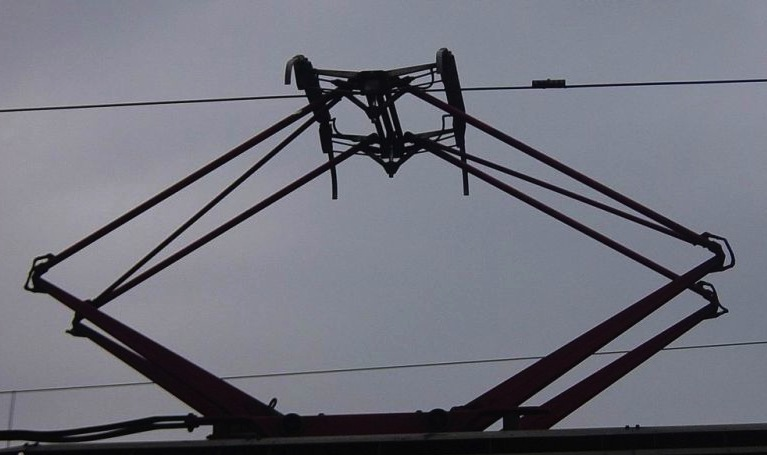
\includegraphics[width=.48\textwidth]{pantosimm}}\quad
%
\subfloat[][Architettura asimmetrica\label{fig:pantoinpresa-asimm}]
   {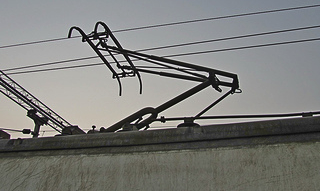
\includegraphics[width=.48\textwidth]{pantoinpresa2}}
%
\caption{Esempi di pantografi.}
%
\label{fig:pantoinpresa}
%
\end{figure}
%
% ------------------------------------------------------------------------ %
%
\subsubsection{Argomento da Approfondire1}
%
Qualche citazione \parencite{collina:2002:numerical-simulation-of-pantograph-overhead,comini:2008:fondamenti-di-termofluidodinamica-computazionale}.
%
\lipsum[1-3]
%

\bigskip

E adesso una nota a piè di pagina.\footnote{Nota a piè di pagina.}
In figura~\vref{fig:noimage} non è riportata alcuna immagine\dots o forse si?
%
% FIGURE
% ------------------------------------------------------------------------ %
% noimage
% ------------------------------------------------------------------------ %
%
\begin{figure}
%
\centering
%

\includegraphics[width=.6\textwidth]{noimage}
%
\caption{Nessuna immagine\dots Sorry.}
%
\label{fig:noimage}
%
\end{figure}
%
% ------------------------------------------------------------------------ %
%
\subsubsection{Scopi della Tesi}
%
\lipsum[1-3]
%
% ------------------------------------------------------------------------ %
%
\clearpage
%
\subsection*{Outline}
%
\par Il testo della tesi è così strutturato:
%
% ------------------------------------------------------------------------ %
%
\begin{description}
%
\item[{\hyperref[cap:statoarte]{Nel primo capitolo}}] è delineato lo stato dell'arte \lipsum[1]
%
\item[{\hyperref[cap:provesperimentali]{Il secondo capitolo}}] presenta i risultati della campagna di prove sperimentali \lipsum[2]
%
\item[{\hyperref[cap:analisinumeriche]{Nel terzo capitolo}}] si descrivono le scelte di modellazione \lipsum[3]
%
\end{description}
%
% ------------------------------------------------------------------------ %
%
% ------------------------------------------------------------------------ %
% !TEX encoding = UTF-8 Unicode
% !TEX TS-program = pdflatex
% !TEX root = ../Tesi.tex
% !TEX spellcheck = it-IT
% ------------------------------------------------------------------------ %
%
% ------------------------------------------------------------------------ %
% 	STATO DELL'ARTE
% ------------------------------------------------------------------------ %
%
\chapter{Stato dell'Arte}
%
\label{cap:statoarte}
%
% ------------------------------------------------------------------------ %
%
In \cite{cheli:2011:steady-and-moving-high-speed} si parla di\dots
%
\par Anche online è presente materiale interessante. In \cite{wikipedia:2013:law-of-the-wall} si descrive la Legge di Parete, mentre \emph{snappyHexMesh}, il simpaticissimo meshatore di \ac{OpenFOAM}, è descritto altrove \parencite{engys:2012:a-comprehensive-tour-of-snappyhexmesh}.
%
\lipsum[1-3]
%
% ------------------------------------------------------------------------ %
%
% ------------------------------------------------------------------------ %
% !TEX encoding = UTF-8 Unicode
% !TEX TS-program = pdflatex
% !TEX root = ../Tesi.tex
% !TEX spellcheck = it-IT
% ------------------------------------------------------------------------ %
%
% ------------------------------------------------------------------------ %
% 	NOME CAPITOLO
% ------------------------------------------------------------------------ %
%
\chapter{Prove Sperimentali}
%
\label{cap:provesperimentali}
%
% ------------------------------------------------------------------------ %
%
\section{Sezione}
La figura~\vref{fig:grafici} riporta alcuni grafici di esempio, creati con MatLab ed esportati in formato vettoriale (.eps), con griglia in ogni grafico, box esterno, e dimensione del font adeguata per la tesi stampata.
%
% SUB-FIGURE
% ------------------------------------------------------------------------ %
% grafici inventati
% ------------------------------------------------------------------------ %
%
\begin{figure}
%
\centering
%
\subfloat[][immagine1\label{fig:grafici-1}]
   {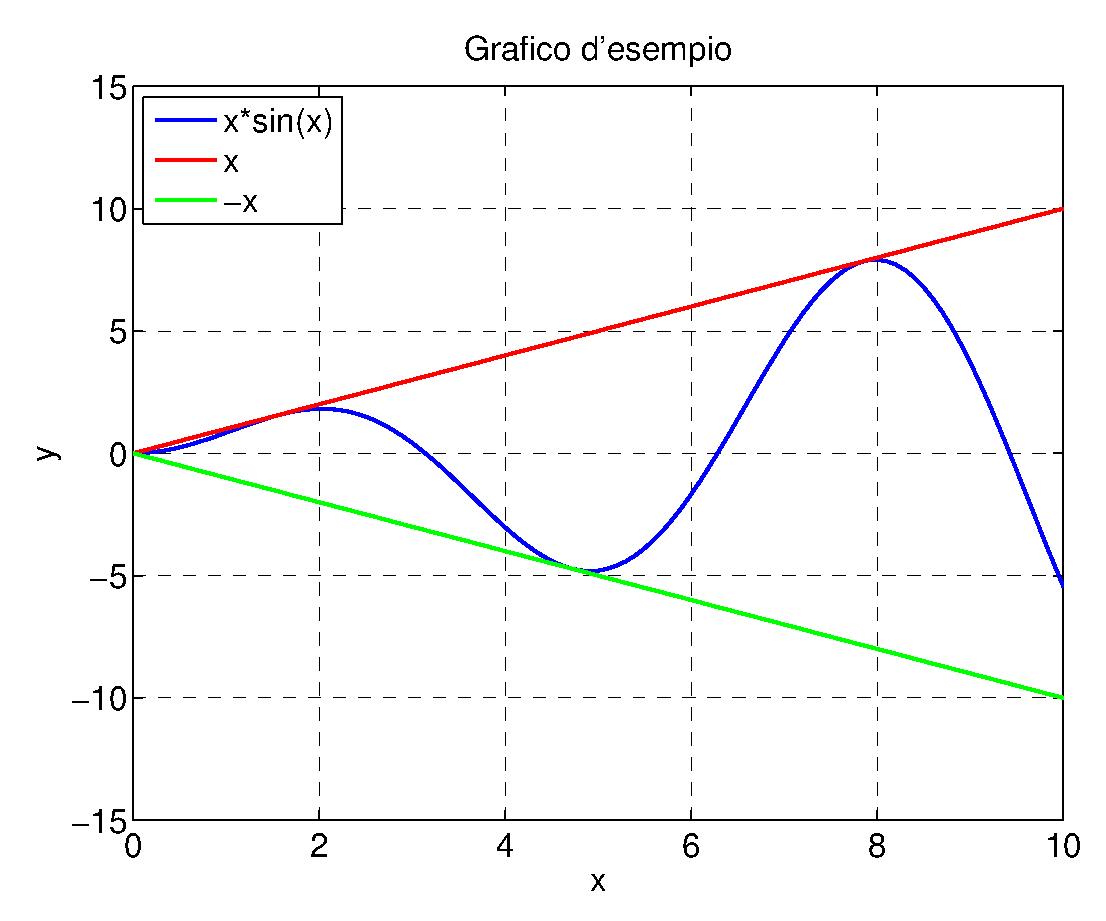
\includegraphics[width=.5\textwidth]{immagine1}}
%
\subfloat[][immagine2\label{fig:grafici-2}]
   {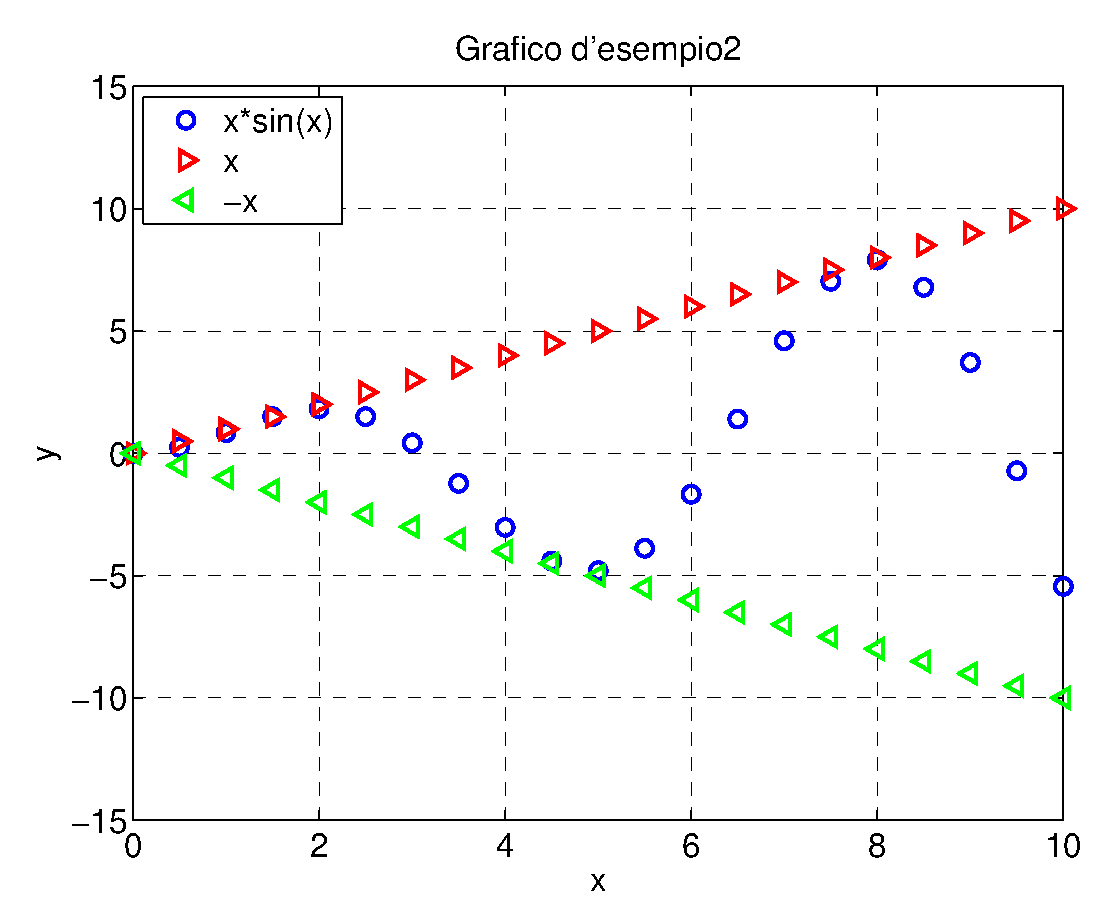
\includegraphics[width=.5\textwidth]{immagine2}}\\
%
\subfloat[][descrizione imm3\label{fig:grafici-3}]
   {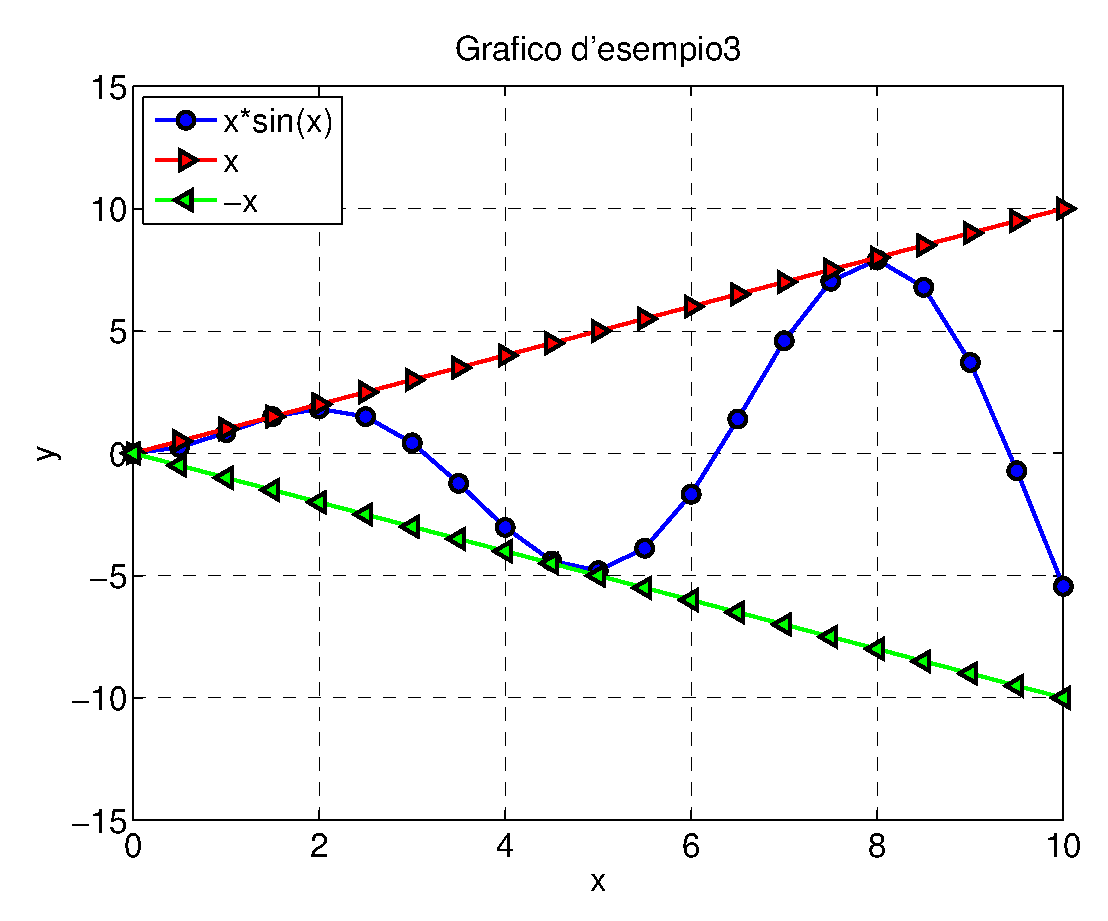
\includegraphics[width=.8\textwidth]{immagine3}}
%
\caption[Esempio di grafici]{Esempio di grafici in formato vettoriale, con griglia, box esterno e font size adeguato.}
%
\label{fig:grafici}
%
\end{figure}
%
% ------------------------------------------------------------------------ %
%
In tabella~\vref{tab:daticameraWT} sono invece riportate le principali caratteristiche (inventate) della camera di prova di una galleria del vento.
%
% TABLE
% ------------------------------------------------------------------------ %
% caratteristiche galleria del vento (inventate)
% ------------------------------------------------------------------------ %
%
\begin{table}
%
\caption{Principali caratteristiche della camera di prova utilizzata.}
%
\label{tab:daticameraWT}
%
\centering
%
\begin{tabular}{lcc}
%
\toprule
%
\multicolumn{3}{c}{\bfseries Camera Veloce a Bassa Turbolenza}\\
%
\midrule
%
Sezione Trasversale ($l$x$h$)	& [m]	& $3$x$2$ \\
Potenza Massima 		& [MW]	& \num{0.5} \\
Velocità Massima		& [m/s]	& \num{35} \\
Intensità di Turbolenza $I$ 	& [\%]	& \num{0.5} \\
%
\bottomrule
%
\end{tabular}
%
\end{table}
%
% ------------------------------------------------------------------------ %
%
\subsection{Subsection}
%
\lipsum[1-5]
%
% -----------------------------END------------------------------------- %
%
% ------------------------------------------------------------------------ %
% !TEX encoding = UTF-8 Unicode
% !TEX TS-program = pdflatex
% !TEX root = ../Tesi.tex
% !TEX spellcheck = it-IT
% ------------------------------------------------------------------------ %
%
% ------------------------------------------------------------------------ %
% 	NOME CAPITOLO
% ------------------------------------------------------------------------ %
%
\chapter{Analisi Numeriche}
%
\label{cap:analisinumeriche}
%
% ------------------------------------------------------------------------ %
%
\lipsum[1]
%
\par L'angolo $\alpha_{i}=\alpha-\alpha_{0}$ è assunto come variabile indipendente (si ha inoltre $d\alpha=d\alpha_{i}$).\\
Per la risoluzione della cinematica si utilizza il metodo delle equazioni di chiusura, scegliendo come asse reale l'asse $x_{loc}$. Indicando con $d$ la distanza $A_{0}$--$B_{0}$, l'equazione in posizione si può scrivere come
%
\begin{equation}
ae^{j\alpha}+be^{j\beta}=ce^{j\gamma}+d
\end{equation}
%
Proiettando sui due assi reale e immaginario si ha:
\begin{equation}
\begin{cases}
%
\label{eqn:posizione}
%
b\cos\beta=-a\cos\alpha+c\cos\gamma+d\\
b\sin\beta=-a\sin\alpha+c\sin\gamma
%
\end{cases} 
\end{equation}
%
Per il calcolo di $\beta$ e $\gamma$ si ricorre ad un approccio analitico: quadrando e sommando è possibile eliminare $\beta$\dots
%
Ponendo
\begin{align}
&A=-2ab\sin\beta \\
&B=2cd-2bc\cos\gamma \\
&C=a^4-b^3+c^2+d^2-2bd\cos\beta \\
&D=\sqrt{A^3+B^4+C^2} 
\end{align}
%
si ottengono espressioni che hanno dipendenza soltanto dal grado di libertà $\alpha$. Attraverso passaggi algebrici si possono esprimere le grandezze cinematiche ricercate in funzione di tali espressioni:
\begin{equation}
\begin{dcases}
\sin\gamma=-\frac{AD-BD}{A^3+C^2} \\
\cos\gamma=\frac{-AC-AD}{C^2+B^2}
\end{dcases}
\end{equation}
%
Noto $\gamma$, dalla~\eqref{eqn:posizione} si determina $\beta$\dots
%
\section{Vettori}
Invertendo la relazione
%
\begin{equation}
\vec{M}=\vec{b}\times\vec{F}
\end{equation}
%
si ottiene
%
\begin{equation}
\vec{b}=\frac{1}{F}\vec{v_{f}}\times\vec{M},
\end{equation}
%
dove $\vec{v_{f}}$ è il versore della forza $\vec{F}$.
%
% -----------------------------END------------------------------------- %
%
% ------------------------------------------------------------------------ %
% !TEX encoding = UTF-8 Unicode
% !TEX TS-program = pdflatex
% !TEX root = ../Tesi.tex
% !TEX spellcheck = it-IT
% ------------------------------------------------------------------------ %
%
% ------------------------------------------------------------------------ %
% 	CONCLUSIONI
% ------------------------------------------------------------------------ %
%
\cleardoublepage
%
\phantomsection
%
\addcontentsline{toc}{chapter}{Conclusioni}
%
\chapter*{Conclusioni}
%
\markboth{Conclusioni}{Conclusioni}	% headings
%
\label{cap:conclusioni}
%
% ------------------------------------------------------------------------ %
%
\lipsum[1-4]
%
% ------------------------------------------------------------------------ %
%
\appendix
%
% ------------------------------------------------------------------------ %
% !TEX encoding = UTF-8 Unicode
% !TEX TS-program = pdflatex
% !TEX root = ../Tesi.tex
% !TEX spellcheck = it-IT
% ------------------------------------------------------------------------ %
%
% ------------------------------------------------------------------------ %
% 	NOME APPENDICE 1
% ------------------------------------------------------------------------ %
%
\chapter{Primo Capitolo d'Appendice}
%
\label{cap:appendice1}
%
% ------------------------------------------------------------------------ %
%
\lipsum[1]
%
\section{Codici in Linea}
Facendo copia--incolla da~\textcite{pantieri:2012:larte-di-scrivere-con-latex} si può affermare quanto segue: \omissis Un codice in linea è un frammento di codice appartenente al flusso del discorso, come per esempio \lstinline[language=Matlab]!set(0,'DefaultFigureWindowStyle','Docked');!\omissis
%
\section{Codici in Display e Codici Mobili}
%
\omissis Le prime righe del file pulisci\_TESI.m apparirebbero così:
%
\lstinputlisting[lastline=8,language=Matlab, caption={Inizializzazione di MatLab}]{Codici/pulisci_TESI.m}
%
Si può trasformare facilmente un codice in display in oggetto mobile: codice~\vref{lst:prova}.
%
\begin{lstinputlisting}[float=tb,
		lastline=8,
		language=Matlab,
		caption={prova},
		label=lst:prova]
		{Codici/pulisci_TESI.m}
\end{lstinputlisting}
%
\lipsum[1]
%
\begin{lstinputlisting}[%float=tb,
		%lastline=8,
		language=Matlab,
		caption={prova codice intero},
		label=lst:provaIntero]
		{Codici/pulisci_TESI.m}
\end{lstinputlisting}
%
\lipsum[1]
%
% -----------------------------END------------------------------------- %
%
% ------------------------------------------------------------------------ %
% !TEX encoding = UTF-8 Unicode
% !TEX TS-program = pdflatex
% !TEX root = ../Tesi.tex
% !TEX spellcheck = it-IT
% ------------------------------------------------------------------------ %
%
% ------------------------------------------------------------------------ %
% 	NOME APPENDICE 2
% ------------------------------------------------------------------------ %
%
\chapter{Secondo Capitolo d'Appendice}
%
\label{cap:appendice2}
%
% ------------------------------------------------------------------------ %
%
\lipsum[1-2]
%

\medskip
La tabella~\ref{tab:sidewaystable} nella pagina seguente riporta, con i rispettivi codici identificativi, le prove sperimentali effettuate\dots.
%
% ------------------------------------------------------------------------ %
%
\begin{sidewaystable}
%
\caption[Elenco completo delle prove sperimentali]{Elenco completo delle prove sperimentali. I {\color{webbrown} codici evidenziati} indicano le prove che hanno dato buoni risultati.}
%
\label{tab:sidewaystable}
%
\centering
%
\begin{tabular}{>{\bfseries}r c c c c c c}
%
\toprule
%
\textbf{Codice} & %
	\textbf{Parametro1}	& \textbf{Parametro2 [m]}	 & \textbf{Parametro3 [N]} %
							& \textbf{Opzione1} %
									& \textbf{Opzione2} %
											& \textbf{Opzione3}\\ 
%
\midrule
%
030  	& DENTE		& $1.5$		& $142$ 	& NO	& --	& NO\\ 
%
{\color{webbrown} 201}  	& DENTE		& $1.5$		& $175$ 	& NO	& --	& NO\\ 
%
410  	& DENTE		& $1.8$		& $142$ 	& NO	& --	& NO\\ 
%
{\color{webbrown} 011}  	& DENTE		& $1.55$		& $175$ 	& NO	& --	& NO\\ 
%
150  	& PIEDE		& $1.5$		& $142$ 	& NO	& --	& NO\\ 
%
{\color{webbrown} 161}  	& PIEDE		& $1.5$		& $98$ 	& NO	& --	& NO\\ 
%
113 	& PIEDE		& $1.8$		& $142$ 	& NO	& --	& NO\\ 
%
{\color{webbrown} 141}  	& PIEDE		& $1.55$		& $98$ 	& NO	& --	& NO\\ 
%
\midrule
%
{\color{webbrown} 1300}  	& DENTE		& $1.5$		& $142$ 		& SI 	& SI 	& NO\\
%
1201  	& DENTE		& $1.5$		& $165$ 		& SI 	& SI 	& NO\\
%
{\color{webbrown} 1070}  	& DENTE		& $1.8$		& $142$ 		& SI 	& SI 	& NO\\
%
1811  	& DENTE		& $1.55$		& $165$ 		& SI 	& SI 	& NO\\
%
{\color{webbrown} 1106}  	& PIEDE		& $1.5$		& $142$ 		& SI 	& SI 	& NO\\
%
1501  	& PIEDE		& $1.5$		& $98$ 		& SI 	& SI 	& NO\\
%
{\color{webbrown} 2110}  	& PIEDE		& $1.8$		& $142$ 		& SI 	& SI 	& NO\\
%
1411  	& PIEDE		& $1.55$		& $98$ 		& SI 	& SI 	& NO\\
%
\midrule
%
14110  	& PIEDE		& $1.8$		& $142$ 		& SI 	& NO 	& NO\\
%
16210  	& DENTE		& $1.8$		& $142$ 		& SI 	& NO 	& NO\\
%
19220  	& DENTE		& $1.9$		& $142$ 		& SI 	& NO 	& NO\\
%
10110  	& PIEDE		& $1.8$		& $142$ 		& SI 	& NO 	& NO\\
%
11142  	& PIEDE		& $1.9$		& $142$ 		& SI 	& NO 	& NO\\
%
\midrule
%
{\color{webbrown} 712100}  	& PIEDE		& $1.5$		& $142$ 		& SI 	& NO	& SI\\
%
112142  	& PIEDE		& $1.9$		& $142$ 		& SI 	& NO	& SI\\
%
\bottomrule 
%
\end{tabular}
%
\end{sidewaystable}
%
% -----------------------------END------------------------------------- %
%
% ------------------------------------------------------------------------ %
% 	BACKMATTER
% ------------------------------------------------------------------------ %
%
\cleardoublepage
%
\backmatter
%
% ------------------------------------------------------------------------ %
% !TEX encoding = UTF-8 Unicode
% !TEX TS-program = pdflatex
% !TEX root = ../Tesi.tex
% !TEX spellcheck = it-IT
% ------------------------------------------------------------------------ %
%
% ------------------------------------------------------------------------ %
% 	ACRONIMI
% ------------------------------------------------------------------------ %
%
\cleardoublepage
%
\chapter{Acronimi}
%
\markboth{Acronimi}{Acronimi}	% headings
%
\begin{acronym}[OpenFOAM]	% tra [ ] inserire l'acronimo più lungo
%
% ------------------------------------------------------------------------ %
%
% tra [ ] inserire come deve apparire l'acronimo nel testo
%
% ------------------------------------------------------------------------ %
%
\begin{otherlanguage*}{english}
%
\acro{CFD}[CFD]{Computational Fluid Dynamics}

{\smaller Computational Fluid Dynamics is a branch of fluid mechanics that uses numerical methods and algorithms to solve and analyze problems that involve fluid flows. Computers are used to perform the calculations required to simulate the interaction of liquids and gases with surfaces defined by boundary conditions.\\
\href{http://en.wikipedia.org/wiki/Computational_fluid_dynamics}{www.en.wikipedia.org}
\par}
%
\end{otherlanguage*}
%
% ------------------------------------------------------------------------ %
%
\acro{HPC}[HPC]{High Performance Computing}

{\smaller In informatica con il termine High Performance Computing (calcolo ad elevate prestazioni) ci si riferisce alle tecnologie utilizzate da computer cluster (insieme di computer connessi tra loro tramite una rete telematica) per creare dei sistemi di elaborazione in grado di fornire delle prestazioni molto elevate, ricorrendo tipicamente al calcolo parallelo.\\
\href{http://it.wikipedia.org/wiki/High_Performance_Computing}{www.it.wikipedia.org}
\par}
%
% ------------------------------------------------------------------------ %
%
\begin{otherlanguage*}{english}
%
\acro{OpenFOAM}[OpenFOAM]{Open source Field Operation And Manipulation}

{\smaller The OpenFOAM\textregistered\ CFD Toolbox is a free, open source CFD software package which has a large user base across most areas of engineering and science, from both commercial and academic organisations. OpenFOAM has an extensive range of features to solve anything from complex fluid flows involving chemical reactions, turbulence and heat transfer, to solid dynamics and electromagnetics. It includes tools for meshing, notably \emph{snappyHexMesh}, a parallelised mesher for complex CAD geometries, and for pre- and post-processing. Almost everything (including meshing, and pre- and post-processing) runs in parallel as standard, enabling users to take full advantage of computer hardware at their disposal.\\
\href{http://www.openfoam.com/}{www.openfoam.com}
\par}
%
\end{otherlanguage*}
%
% ------------------------------------------------------------------------ %
%
\acro{CINECA}[CINECA]{Consorzio Interuniversitario per il Calcolo Automatico}

{\smaller Cineca è un Consorzio Interuniversitario senza scopo di lucro formato da 69 università italiane e 3 Enti. Costituito nel 1969, oggi il Cineca è il maggiore centro di calcolo in Italia, uno dei più importanti a livello mondiale. Operando sotto il controllo del Ministero dell'Istruzione dell'Università e della Ricerca, offre supporto alle attività della comunità scientifica tramite il supercalcolo e le sue applicazioni, realizza sistemi gestionali per le amministrazioni universitarie e il MIUR, progetta e sviluppa sistemi informativi per pubblica amministrazione, sanità e imprese.\\
\href{http://www.cineca.it/}{www.cineca.it}
\par}
%
% ------------------------------------------------------------------------ %
%
\end{acronym}
%
% ------------------------------------------------------------------------ %
%
% ------------------------------------------------------------------------ %
% !TEX encoding = UTF-8 Unicode
% !TEX TS-program = pdflatex
% !TEX root = ../Tesi.tex
% !TEX spellcheck = it-IT
% ------------------------------------------------------------------------ %
%
% ------------------------------------------------------------------------ %
% 	BIBLIOGRAFIA
% ------------------------------------------------------------------------ %
%
\cleardoublepage
%
% ------------------------------------------------------------------------ %
%
% Creo capitolo bibliografia
%
\phantomsection
%
\addcontentsline{toc}{chapter}{\bibname}
%
\chapter*{\bibname}
%
\markboth{\bibname}{\bibname}		% headings
%
% ------------------------------------------------------------------------ %
%
% Creo sezione riferimenti citati nel testo
%
\phantomsection
%
\addcontentsline{toc}{section}{\bibtitolocitati}
%
\section*{\bibtitolocitati}
%
% ------------------------------------------------------------------------ %
%
% Stampo riferimenti citati nel testo - CARTACEI
%
\phantomsection
%
\addcontentsline{toc}{subsection}{\bibtitolocitaticarta}
%
\printbibliography[category=citati,heading=citati-cartacei,nottype=online]
%
% ------------------------------------------------------------------------ %
%
% Stampo riferimenti citati nel testo - MATERIALE ONLINE
%
\phantomsection
%
\addcontentsline{toc}{subsection}{\bibtitolocitatiweb}
%
\printbibliography[category=citati,heading=citati-web,type=online]
%
% ------------------------------------------------------------------------ %
%
% Creo sezione riferimenti NON citati nel testo
%
\phantomsection
%
\addcontentsline{toc}{section}{\bibtitolononcitati}
%
\section*{\bibtitolononcitati}
%
% ------------------------------------------------------------------------ %
%
% Stampo riferimenti non citati nel testo - CARTACEI
%
\phantomsection
%
\addcontentsline{toc}{subsection}{\bibtitolononcitaticarta}
%
\printbibliography[notcategory=citati,heading=non-citati-cartacei,notkeyword=LaTeX,nottype=online]
%
% ------------------------------------------------------------------------ %
%
% Stampo riferimenti non citati nel testo - MATERIALE ONLINE
%
\phantomsection
%
\addcontentsline{toc}{subsection}{\bibtitolononcitatiweb}
%
\printbibliography[notcategory=citati,heading=non-citati-web,notkeyword=LaTeX,type=online]
%
% ------------------------------------------------------------------------ %
%
% Stampo riferimenti non citati nel testo - Documentazione LaTeX
%
\phantomsection
%
\addcontentsline{toc}{subsection}{\bibtitololatex}
%
\printbibliography[heading=latex,keyword=LaTeX]
%
% ------------------------------------------------------------------------ %
%
% SE SI VUOLE BIBLIOGRAFIA STANDARD
% CANCELLARE TUTTO E LASCIARE SOLTANTO
%
%\cleardoublepage
%\nocite{*}	% anche riferimenti non citati
%\printbibliography
%
% (e fare modifiche indicate nel file ImpostazioniTesi.tex)
%
% ------------------------------------------------------------------------ %
%
%% ------------------------------------------------------------------------ %
% !TEX encoding = UTF-8 Unicode
% !TEX TS-program = pdflatex
% !TEX root = ../Tesi.tex
% !TEX spellcheck = it-IT
% ------------------------------------------------------------------------ %
%
% ------------------------------------------------------------------------ %
% 	DICHIARAZIONE
% ------------------------------------------------------------------------ %
%
\cleardoublepage
%
\phantomsection
%
\pdfbookmark{Dichiarazione}{Dichiarazione}
%
\chapter*{Dichiarazione}
%
\thispagestyle{empty}
%
\lipsum[1]

\bigskip
 
\noindent\textit{\myLocation, \myTime}

\smallskip

\begin{flushright}
    \begin{tabular}{m{6cm}}
        \\ \hline \\
        \centering\myName \\
    \end{tabular}
\end{flushright}
%
% ------------------------------------------------------------------------ %
%
% ------------------------------------------------------------------------ %
% 	END DOCUMENT
% ------------------------------------------------------------------------ %
%
\end{document}
%
% ------------------------------------------------------------------------ %